\begin{center}
\Large \textbf{Problema I} \\
\say{\texttt{caminos}}
\end{center}

Comenzando en la esquina superior izquierda de un tablero de $2 \times 2$, y pudiendo moverse solamente hacia la derecha y hacia abajo,
hay exactamente $6$ caminos hasta la esquina inferior derecha.

\begin{figure}[H]
    \centering
    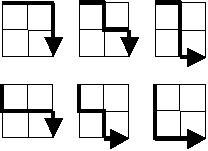
\includegraphics[width=0.3\textwidth]{Imagenes/Stock/Caminos en grilla.png}
\end{figure}

\underline{¿Cuántos caminos de este tipo hay a través de un tablero de $5 \times 5$?}

